\documentclass[12pt,letterpaper]{article}

%Trennungsregeln etc.
\usepackage[english]{babel}

%Schriftart
%see http://www.tug.dk/FontCatalogue/ for more
%Ideen: baskervald
%for working: arev
\usepackage{baskervald}

%Sonderzeichenein-/ausgabe (http://tex.stackexchange.com/questions/44694/fontenc-vs-inputenc for questions)
\usepackage[utf8]{inputenc}
\usepackage[T1]{fontenc}

%Zeilenabstand, Optionen: singlespacing, onehalfspacing, doublespacing
\usepackage[onehalfspacing]{setspace}

%Seitenränder, hier oneside
\usepackage[left=2.5cm,right=2.5cm,top=2.5cm,bottom=2.5cm]{geometry}

%Anführungszeichen (for help see CTAN-package-page:  http://ftp.gwdg.de/pub/ctan/macros/latex/contrib/csquotes/csquotes.pdf)
\usepackage[strict=true,autostyle=true,german=quotes]{csquotes}

%Einrücklänge der ersten Zeile eines neuen Absatzes, standardmäßig drin
\setlength{\parindent}{1cm}

%Seitenzahlen
\usepackage{scrlayer-scrpage}
\pagestyle{scrheadings}
\ofoot[]{\pagemark}

%%Chapter/Section-Überschriften (Schriftart, Größe)
%Section-Überschriften
%\setkomafont{section}{\normalfont \bfseries \Large} 
%Inhaltsverzeichnis auch mit Serifen
%\setkomafont{disposition}{\normalcolor\bfseries}

%for pictures (png)
\usepackage{graphicx}
%\usepackage{float} %jetzt kann man mit H hinter figure fest setzen
\usepackage{wrapfig}
\usepackage[font={small,it}]{caption}

%insert hyperlinks
\usepackage[colorlinks=true, urlcolor=blue, linkcolor=black, citecolor = black]{hyperref}
\usepackage{url}

%Literaturverzeichnis
\usepackage[author year]{natbib}

%insert codesnippets
%\usepackage{listings}
%\usepackage{xcolor}
%\definecolor{deepblue}{rgb}{0,0,0.5}
%\definecolor{deepred}{rgb}{0.6,0,0}
%\definecolor{deepgreen}{rgb}{0,0.5,0}
%\lstset{ 
%	language=Python, % choose the language of the code
%	commentstyle=\itshape\color{yellow},
%	basicstyle=\fontfamily{pcr}\selectfont\footnotesize\color{white},
%	otherkeywords={self},
%	keywordstyle=\color{violet}\bfseries, % style for keywords
%	emph={MyClass,__init__},          % Custom highlighting
%	emphstyle=\color{cyan},    % Custom highlighting style
%	stringstyle=\color{deepgreen}
%	numbers=none, % where to put the line-numbers
%	numberstyle=\tiny, % the size of the fonts that are used for the line-numbers     
%	backgroundcolor=\color{black},
%	showspaces=false, % show spaces adding particular underscores
%	showstringspaces=false, % underline spaces within strings
%	showtabs=false, % show tabs within strings adding particular underscores
%	frame=single, % adds a frame around the code
%	tabsize=2, % sets default tabsize to 2 spaces
%	rulesepcolor=\color{gray},
%	rulecolor=\color{black},
%	captionpos=b, % sets the caption-position to bottom
%	breaklines=true, % sets automatic line breaking
%	breakatwhitespace=false,
%	stringstyle=\color{orange}
%}


%Literaturverzeichnis
%\usepackage[author year]{natbib} %hier muss noch komme zwischen Autor und Jahr weg
%\documentclass{article}% use option titlepage to get the title on a page of its own.
\pagestyle{plain}
\usepackage{blindtext}
\title{Colorful Image Colorization with TensorFlow}
\date{\today}
\author{Sophia Schulze-Weddige \and Malin Spaniol \and Maren Born \\Implementing Artificial Neural Networks with Tensorflow \\Universität Osnabrück}
\begin{document}
\maketitle
\thispagestyle{empty}
\newpage
\thispagestyle{empty}
\tableofcontents
\newpage
\section{Introduction}
Based on the paper \emph{Colorful Image Colorization} \citep{Zhang.2016}, this project aims to reimplement a similar artificial neural network which transforms grayscale images into colorful pictures. This task involves creating a dataset based on pictures that are converted into the CIELAB colorspace (\emph{Lab}), such that the lightness channel \emph{L} can be considered as the input whereas the \emph{a} and \emph{b} channels, which encode color information, form the target for the model. We closely rebuild the layers of the original model (they used \enquote{caffe} \citep{jia2014caffe}) using tensorflow 2.0.\\
Our project is divided into two steps, which are also discussed in the paper \citep{Zhang.2016}. In the first step, the unaltered \emph{ab} channels are utilized as the prediction target, applying the mean squared error loss. As predicted by Zhang et al. (2016) this approach favors desaturated colors predicting images to appear sepia or greyish. This approach can be thought of as the \enquote{classical} way of automated image colorization with convolutional neural networks.\\
The second step aims to rebuild the main contribution to the image colorization problem from Zhang et al. (2016), namely to translate the problem to a classification task. By doing so, Zhang et al. (2016) were able to predict more plausible colors for the grayscale images. Due to the lack of time, we were not able to train our models long enough to reproduce the good results provided. More training time will hopefully lead to vivid and realistic colorizations for gray scale images with our model as well.

\section{Theoretical Background}
Image colorization can be used to modernize pictures or movies. There is a wide range of methods, ranging from hand colorization with photoshop to automatic colorization with artificial intelligence. For examples on images colorization see \url{https://www.reddit.com/r/Colorization/}. The TV-series \enquote{Greatest Events of WWII in Colour} states a good example for the usage of colorized footage. They use the techniques such that events appear more contemporary thus the historic incidents turn out even more worrying (\url{https://www.imdb.com/title/tt9103932/}). 
Automating the colorization problem with deep learning seems to be achievable, as training data is easily available.

\subsection{Related work}
Automatic approaches solving the colorization problem mostly differ in acquisition and handling of the data in order to model the accurate correspondence \citep{Zhang.2016}. One can differentiate between parametric and non-parametric approaches. Non-parametric methods predict colors based on one or more reference images. That means the color distribution of the reference images, which are either provided by the user (e.g. Scribble-based colorization by \cite{Levin.2004}) or automatically, is transferred to the target image. Hence, performance depends heavily on the quality of the provided data \citep{Cheng_2015}.\\
Parametric methods on the other hands, learn prediction functions from large datasets of color images. Different methods are available to achieve this, one of which are convolutional neural networks (CNNs) in which the problem can be posed as regression or classification of quantized color values \citep{Zhang.2016}.

\subsection{Convolutional neural networks for image colorization}
Whenever dealing with image data, CNNs are frequently used as model structures for deep learning tasks. They are inspired by the visual cortex of the brain. The idea is that highly specialized components learn a very specific task, which is similar to the receptive fields of neurons in the visual cortex \citep{Hubel1962}. These components can be combined to high-level features, which again can be merged to classes or transformed to the desired output shape. In CNNs, this concept is implemented by several successive convolutional layers: a weight kernel moves over the input image and calculates the new pixel value for each pixel position by multiplying the weights of the kernel with the neighboring pixel values and summing them up (see fig. \ref{convolut}). Different kernels can generate different so-called feature maps. One feature map targets the same feature (e.g. edges) in different image sections.

\begin{wrapfigure}[12]{r}{0.5\textwidth}
	\centering
	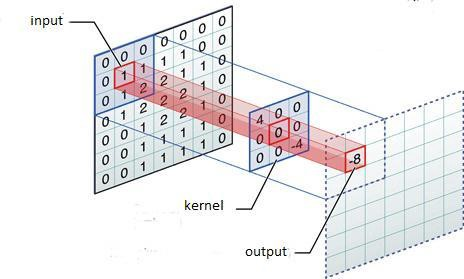
\includegraphics[width=.48\textwidth]{cnn.png}
	\caption{Convolutional operation: kernel slides over the input, multiplying it with its weight before summarizing the 3x3 neighborhood \citep{Escontrela.2018}.}
	\label{convolut}
\end{wrapfigure}
In this manner, CNNs can store spatial information about pixels and features. In a subsequent pooling layer dimensions are reduced by summarizing over the image section (e.g. max pooling takes the highest value of a certain image section). This facilitates the computation and drops unnecessary information \citep{Lecture.2019}. In recent years, CNNs improved such that they outperform humans in many classification tasks \citep{Russakovsky.2014}.

\subsection{Guiding Paper} 
Zhang and colleagues (2016) propose a fully automatic approach to colorize grayscale images. They choose to solve this task with a feed-forward CNN as a classification task using a custom loss and class-rebalancing at training time in order to increase the diversity of the colours in the final results. The model is trained over a million color images from ImageNet dataset \citep{Russakovsky.2014}. Concerning the CNN architecture, they use a single stream, VGG-styled network with added depth and dilated convolutions.\\
The mapping, which Zhang and colleagues (2016) aim to learn, results out of the \emph{Lab} color space: The input is the \emph{L} lightness channel, the target channels are the \emph{a} and \emph{b} color channels. First, they used the Euclidean loss to train the model. This leads to overall grayish colors because the Euclidean loss favors the mean of all color pixel values. Therefore, Zhang et al. (2016) choose to treat the problem as a multinomial classification task. The \emph{ab} output space is therefore divided into bins of grid size ten, and the 313 color values in-gamut span the 313 possible color combinations. Following, a mapping to a probability distribution over all 313 possible colors is learned for each input. The ground truth color is converted to a vector, using a soft-encoding scheme and a multinomial cross entropy loss, which is responsible for the class-rebalancing. Thereafter, they map the probability distribution to the color values. The class-rebalancing operates pixel-wise and the loss of each pixel is re-weighted at training time, based on how often the color occurs.

\section{Networkstructure and Implementation}
The re-implementation of the original paper \citep{Zhang.2016} was conducted in two steps and can be found on GitHub (\url{https://github.com/marumse/colorize_images}). This chapter will explain these two crucial steps in further detail. In both approaches, the ImageNet2012 dataset was used. Firstly, we implemented the model structure as described in the paper (see figure \ref{network}) and trained the model with the color layers of the input images as the target. Secondly, we translated the colorization task to a classification problem and trained the same model structure with the altered problem representation.
\begin{figure}[hb]
	\centering
	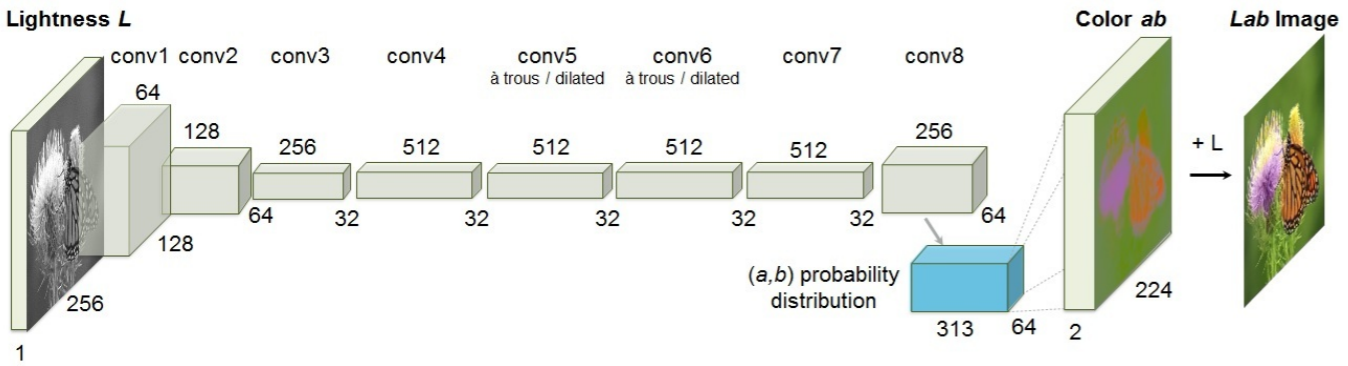
\includegraphics[width=1.0\textwidth]{layer.png}
	\caption{The network architecture of Zhang et al. (2016). }
	\label{network}
\end{figure}
\subsection{Data Generation}
The ImageNet2012 dataset was available to us through the university server. As we were working with a large amount of data in each batch, it would have been impossible to load the whole dataset at once, hence we used a data generator to load the input and target images successively for each batch. Although there are inbuilt data generators available from keras that allow for some means of data augmentation, we built our costum generator to ensure the functionality we were aiming at. The generator takes the batch size and a list which contains the paths to the images that should be used in order to create the input and target arrays as described in the following.\\
\begin{figure}[h]
	\centering
	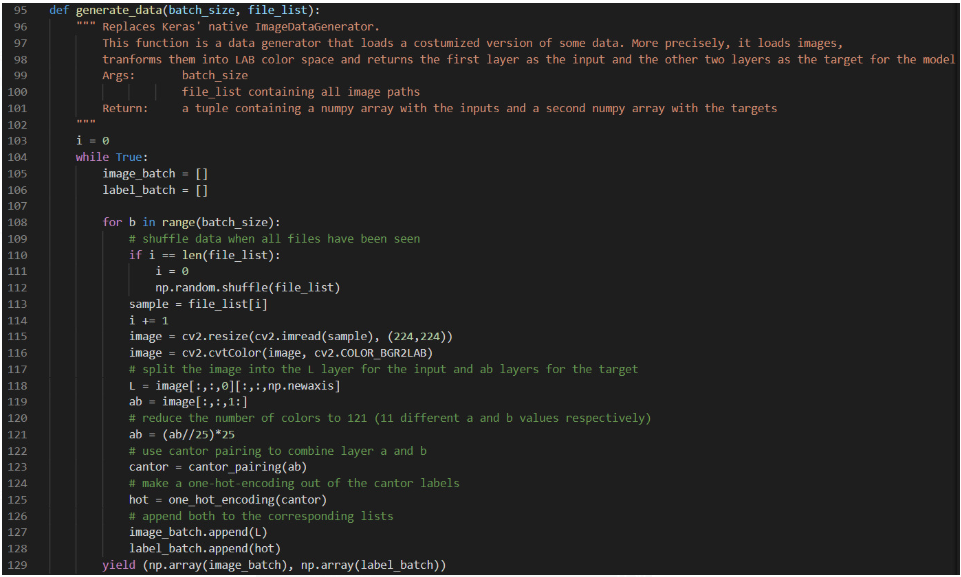
\includegraphics[width=1.0\textwidth]{code_datagen.png}
	\caption{The data generator creates batches of input and target tupels.}
	\label{datagen}
\end{figure}
First, the images are loaded and resized to a uniform shape of (224, 224, 3), which corresponds to the height, the width and the number of the color channels, respectively. Then, the images are transformed from BGR to \emph{Lab} color space. The lightness channel (\emph{L}-layer), which displays most of the structure, is separated from the other two channels and used as the input for the model. The remaining two channels (\emph{ab}-layers) encode the color information of the images and are used as the models’ target in the first approach. In the second approach, these processing steps remain the same. Additionally the target arrays are transformed to become a classification task.\\
The classification task is done in three main steps. The first step is to discretize the continuous color space and reduce the number of possible colors by quantizing the a and b color ranges into eleven bins each. This yields a total of 121 possible colors by combining the a and b layers. In the second step, the a and b layers are combined into a single layer, which keeps the same height and width dimensions as before. This means that the color information of each pixel is now encoded in a single number rather than two, which leads to a single target layer. Cantor pairing is used to generate a unique and deterministic number from the two a and b values of each pixel. The Cantor pairing formula is shown in (1) and its implementation in figure \ref{cantorpairing}. As cantor pairing is reversible, one can easily translate the pairing result back to the original color values with no loss of information \citep{cantor2007}.\\
\begin{equation}
z = \pi(x,y) = \frac{(x+y+1)(x+y)}{2}+y
\end{equation}\\
\begin{figure}[h]
	\centering
	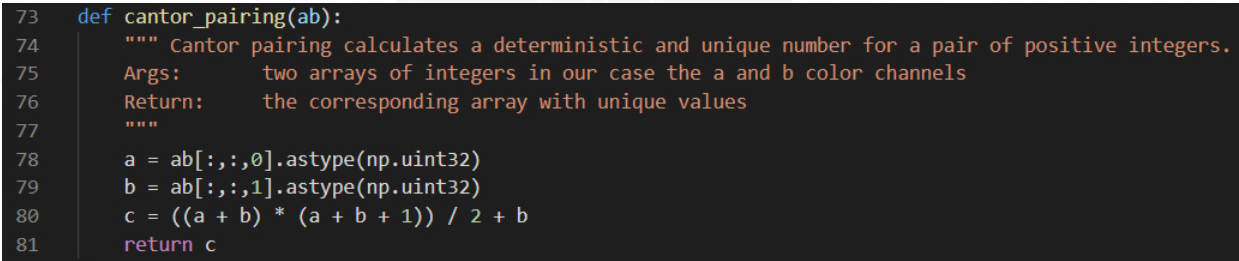
\includegraphics[width=1.0\textwidth]{code_cantor_pairing.png}
	\caption{Implementation of the Cantor Pairing Function.}
	\label{cantorpairing}
\end{figure}
Now that there is a single value encoding each pixels’ color, the third and last step is to translate this value into a one-hot encoding. With the help of a dictionary, the cantor values are translated to numbers from 0 to 120. These numbers serve as the index in the one-hot encoding. Hence, color values that were previously represented in two values (\emph{a} and \emph{b} color channels) are now encoded by their index in the one-hot encoding. The target array has a shape of (224, 224, 121) and a one-hot vector is located at each pixel position.
\begin{figure}[htb]
	\centering
	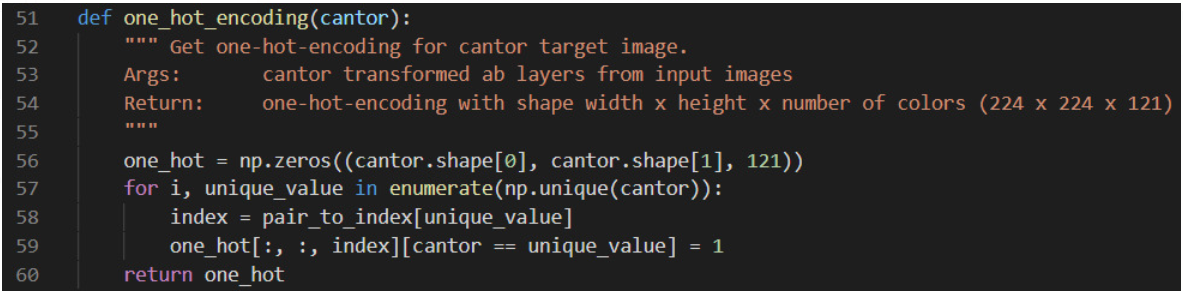
\includegraphics[width=1.0\textwidth]{code_onehot.png}
	\caption{Implementation of the one-hot encoding.}
	\label{onehot}
\end{figure}

\subsection{Modelstructure}
The model structure is equivalent to the original implementation by Zhang et al. (2016). Only minor changes occur, mostly due to the translation from caffe to keras. The model consists of eight blocks comprising two or three repeated convolution and ReLU activation layers followed by a batch normalization. There are no pooling layers in the model, as changes  in  resolution  are  achieved  through  spatial  down-  or  upsampling between the convolution blocks. A transposed convolutional layer is used to inverse the convolution and upsample the output back to the correct size.\\
In the first approach, a stochastic gradient descent optimizer (SGD) with a learning rate of 0.001 and a momentum of 0.9 is used, which is inspired by the original paper. SGD is a stochastic approximation to gradient descent, which uses an estimation for the gradients and thereby decreases the computational complexity. In each optimization step, a random data point is selected from which the gradients are calculated rather than using the whole dataset. The downside to SGD is that it does not guarantee to converge to a solution as the gradients might vary heavily from sample to sample \citep{Lecture.2019}. Further,  mean squared error (MSE) is implemented as the loss function, which uses the average squared difference between the estimated and the target values (2). In the case of image data, that means that each estimated pixel value is compared to the target pixel value and the average over the squared differences is used to optimize the estimation process.
\begin{equation}
MSE = \frac{1}{n}\sum_{i=1}^N(y_i - \tilde{y_i})^2
\end{equation}
\\
In the second approach, the softmax activation function is used in the last layer to prepare the model’s output for the categorical cross entropy loss (3), which compares the output vector ($\tilde{y}$) to the one-hot encoded target vector ($y$).
\begin{equation}
L(y,\tilde{y}) = -\sum_{j=0}^M \sum_{i=0}^N
{{y_i}_j}*log({\tilde{y_i}_j})
\end{equation}
\\
Both, SGD and Adam optimizer are tested. In the two approaches, kernel weights are initialized with the glorot uniform initializer which draws samples from a uniform distribution depending on the number of input and output units of the corresponding weight tensor. Biases are initialized with zeros.

%- image preprocessing documentation\\
%\url{https://keras.io/preprocessing/image/#imagedatagenerator-class}\\
%- preprocessing via ImageDataGenerator() from keras.prepeocessing.image\\
%- takes in traindata, validation data and test data\\
%- featurewise-center and featurewise std\\
%- classmode: none -> is for predictions\\

\subsection{Training}
The models were trained on the grid of the institute of Cognitive Science at Osnabrueck University. A helper script was written that distributed several grid jobs on different computers in order to experiment with the hyperparameters such as the learning rate and the batch size. Through this script, one can easily change these parameters as well as select the data set in addition to the environment and switch between the training mode and the prediction mode. The models were trained with 2000 images and batch sizes of 10 or 20 images. The learning rate varied from 0.1 to 0.001.

\subsection{Testing}
To evaluate the predictive power of our two approaches, colors for unseen test images are predicted and evaluated via visual inspection. When the script is started in prediction mode, the model is not trained, but the weights from the corresponding training process are loaded. The model then predicts the most plausible colors for the L-layer of each input image. In the first approach, the model's output can be interpreted as the ab layers. That means the output can be combined with the input (L-layer) and displayed as an image straight away. For the second approach, three decoding steps are necessary before generating human-readable images. Firstly, the output of the softmax layer is decoded to find the index of the most likely color value. Secondly, this index is translated to the cantor pairing value it represents with the help of the created dictionary. And thirdly, the cantor pairing value is transformed back to the a and b values it is originally constituted of. These a and b layers can finally be combined with the L-layer to display the predicted image in Lab color space.
\section{Results}
\subsection{Classical Approach}
\begin{figure}
	\centering
	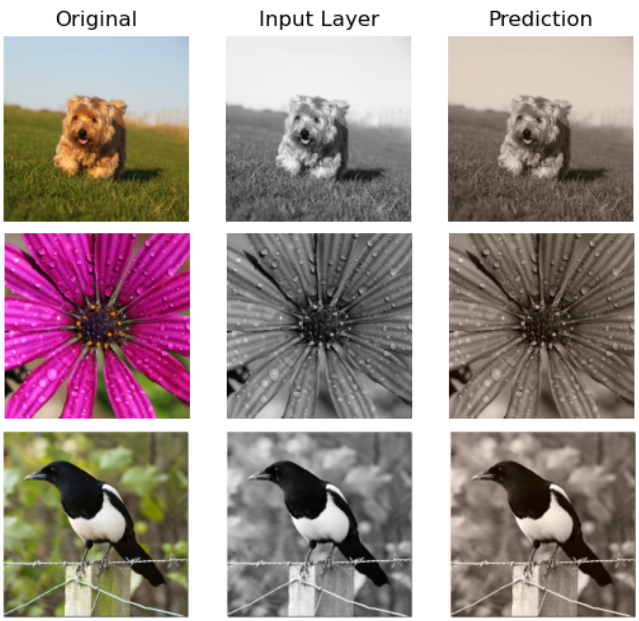
\includegraphics[width=0.8\textwidth]{class_predict.png}
	\caption{}
	\label{class}
\end{figure}

\begin{figure}[h!]
	\centering
	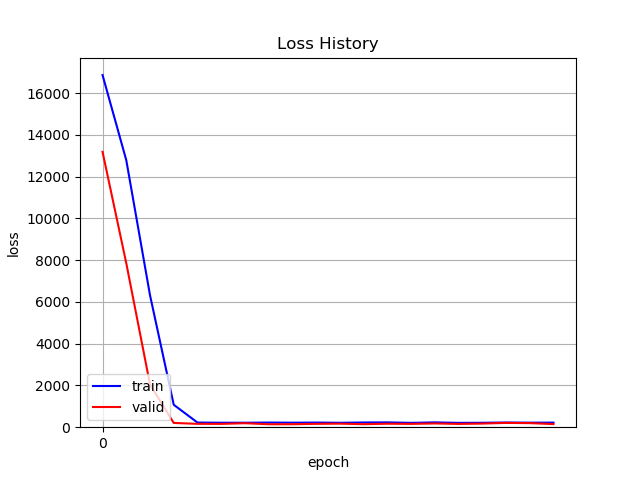
\includegraphics[width=0.8\textwidth]{loss_classical.png}
	\caption{}
	\label{loss_class}
\end{figure}

\subsection{Classification Approach}
\begin{figure}
	\centering
	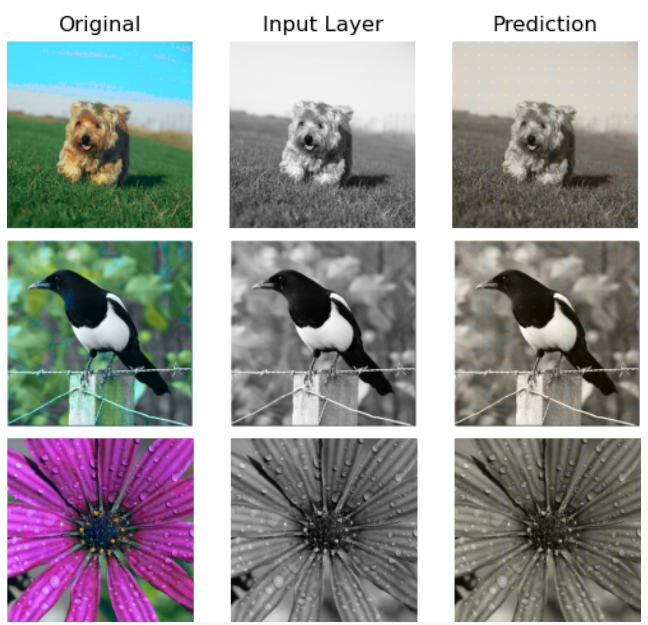
\includegraphics[width=0.8\textwidth]{classific_predict.png}
	\caption{}
	\label{class}
\end{figure}

\section{Discussion}

\subsection{Conclusion and Future Work}
- vergleich ziehen zu Zhang\\
\newpage
\thispagestyle{empty}
\section{Literature}
\label{Lit}
\bibliographystyle{apa}
\renewcommand{\bibsection}{}

\bibliography{lit}

\newpage
\appendix
\automark[section]{section}
\section{Errors}
\begin{figure}[ht]
	\centering
	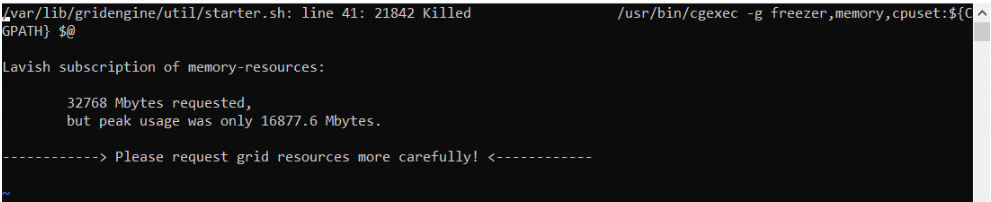
\includegraphics[width=1.0\textwidth]{error.png}
	\caption{}
	\label{error}
\end{figure}

	
\end{document}
